\documentclass[10pt,ignorenonframetext,aspectratio=169,notes=hide,]{beamer}
\usetheme{paloalto}
\usefonttheme{professionalfonts}
\setbeamertemplate{caption}[numbered]
\setbeamertemplate{caption label separator}{: }
\setbeamercolor{caption name}{fg=normal text.fg}
\usepackage{amssymb,amsmath}

\usepackage{ifxetex,ifluatex}
\usepackage{fixltx2e} % provides \textsubscript
\usepackage{lmodern}
%\usepackage{xecjk}
\ifxetex
  \usepackage{fontspec,xltxtra,xunicode}
  \defaultfontfeatures{Mapping=tex-text,Scale=MatchLowercase}
  \newcommand{\euro}{€}
\else
  \ifluatex
    \usepackage{fontspec}
    \defaultfontfeatures{Mapping=tex-text,Scale=MatchLowercase}
    \newcommand{\euro}{€}
  \else
    \usepackage[T1]{fontenc}
    \usepackage[utf8]{inputenc}
      \fi
\fi
% use upquote if available, for straight quotes in verbatim environments
\IfFileExists{upquote.sty}{\usepackage{upquote}}{}
% use microtype if available
\IfFileExists{microtype.sty}{\usepackage{microtype}}{}
\usepackage{longtable,booktabs}
\usepackage{caption}
% These lines are needed to make table captions work with longtable:
\makeatletter
\def\fnum@table{\tablename~\thetable}
\makeatother
\usepackage{url}
\usepackage{graphicx}
\makeatletter
\def\maxwidth{\ifdim\Gin@nat@width>\linewidth\linewidth\else\Gin@nat@width\fi}
\def\maxheight{\ifdim\Gin@nat@height>\textheight0.8\textheight\else\Gin@nat@height\fi}
\makeatother
% Scale images if necessary, so that they will not overflow the page
% margins by default, and it is still possible to overwrite the defaults
% using explicit options in \includegraphics[width, height, ...]{}
\setkeys{Gin}{width=\maxwidth,height=\maxheight,keepaspectratio}

% Comment these out if you don't want a slide with just the
% part/section/subsection/subsubsection title:
\AtBeginPart{
  \let\insertpartnumber\relax
  \let\partname\relax
  \frame{\partpage}
}
\AtBeginSection{
  \let\insertsectionnumber\relax
  \let\sectionname\relax
  \frame{\sectionpage}
}
\AtBeginSubsection{
  \let\insertsubsectionnumber\relax
  \let\subsectionname\relax
  \frame{\subsectionpage}
}

\setlength{\parindent}{0pt}
\setlength{\parskip}{6pt plus 2pt minus 1pt}
\setlength{\emergencystretch}{3em}  % prevent overfull lines
\providecommand{\tightlist}{%
  \setlength{\itemsep}{0pt}\setlength{\parskip}{0pt}}
\newcommand{\ct}{\tiny \textcolor{gray}}

\title{Influence of Chinese city's hygiene on SARS-CoV2 transmission}
\subtitle{A retrospective analysis on transmission dynamics}
\author[Wang et al.]{Wanqi Wang}
\institute{Xian Jiaotong-Liverpool University}
\date{2020/06/03 (updated: 2020-06-08)}


%\setbeamertemplate{footline}[page number]
\defbeamertemplate*{footline}{shadow theme}
{%
  \leavevmode%
  \hbox{\begin{beamercolorbox}[wd=.5\paperwidth,ht=2.5ex,dp=1.125ex,leftskip=.3cm plus1fil,rightskip=.3cm]{author in head/foot}%
    \usebeamerfont{author in head/foot}\hfill\insertshortauthor
  \end{beamercolorbox}%
  \begin{beamercolorbox}[wd=.5\paperwidth,ht=2.5ex,dp=1.125ex,leftskip=.3cm,rightskip=.3cm plus1fil]{title in head/foot}%
    \usebeamerfont{title in head/foot}\insertshorttitle\hfill\insertframenumber\,/\,\inserttotalframenumber%
  \end{beamercolorbox}}%
  \vskip0pt%
}

\beamertemplatenavigationsymbolsempty

\setbeamertemplate{note page}[plain]

\begin{document}
\frame{\titlepage}

\begin{frame}{Outline}
\tableofcontents
\end{frame}
\hypertarget{motivation}{%
\section{Motivation}\label{motivation}}

\begin{frame}{Background}
\protect\hypertarget{background}{}

\begin{itemize}
\tightlist
\item
  Transmission dynamics of this emerging infectious disease haven't been fully understanded
\item
  Environment is closely related to human health
\item
  A city's hygiene may have prominent influence of the SARS-CoV2 transmission.
\end{itemize}

\end{frame}

\begin{frame}{My Aim}
\protect\hypertarget{my-aim}{}

\begin{itemize}
\item
  Get the datasets which is sufficent and high-quality to conduct the analysis
\item
  Evaluate how city's hygiene can impact the transmisstion dynamics of SARS-CoV-2.
\end{itemize}

\end{frame}

\begin{frame}{Causality \& Association}
\protect\hypertarget{causality-association}{}

Will eating ice-cream cause flood?

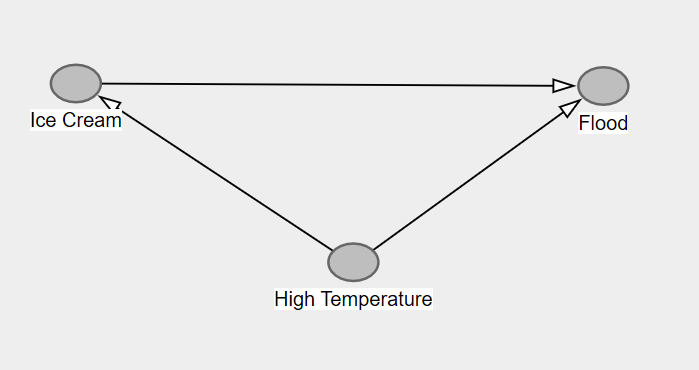
\includegraphics[width=1\linewidth]{image/p1}

\end{frame}

\begin{frame}{Causality \& Association}
\protect\hypertarget{causality-association-1}{}

Any guess of a third variable?

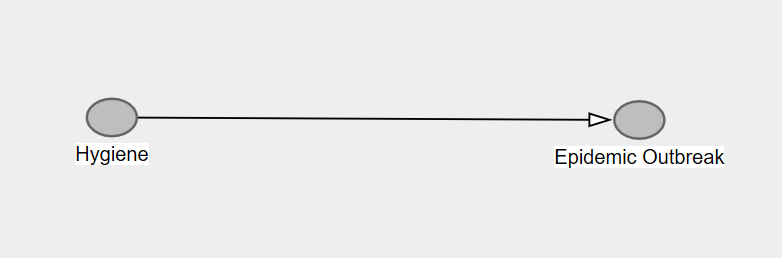
\includegraphics[width=1\linewidth]{image/p1c}

\end{frame}

\begin{frame}{Causality \& Association}
\protect\hypertarget{causality-association-2}{}

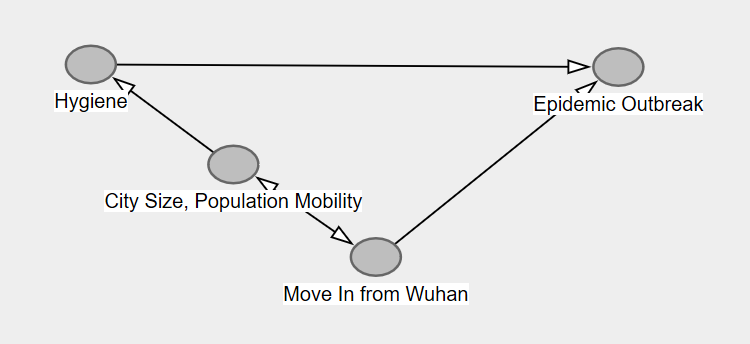
\includegraphics[width=1\linewidth]{image/p2}

\end{frame}

\hypertarget{methods}{%
\section{Methods}\label{methods}}

\begin{frame}{Study Design}
\protect\hypertarget{study-design}{}

\begin{columns}[T]
\begin{column}{0.48\textwidth}
\begin{itemize}
\item
  Retrospective study
\item
  Causal model
\item
  Multi-dataset

  \begin{itemize}
  \tightlist
  \item
    Hygiene Data
  \item
    Epidemic Data
  \item
    Move-out Data
  \end{itemize}
\end{itemize}
\end{column}

\begin{column}{0.48\textwidth}

\includegraphics[width=1\linewidth]{image/p3}
\end{column}
\end{columns}

\end{frame}

\begin{frame}{Measures of Hygiene}
\protect\hypertarget{measures-of-hygiene}{}

\textbf{National hygienic city}
- Ninety three reconfirm national hygienic cities in China in 2018, this is the newested list of national hygienic city.(\href{http://www.chinanews.com/gn/2019/03-20/8785718.shtml}{Source: National Health Commisson of the People's Republic of China; Date: Mar 20th, 2019}).

\begin{itemize}
\item
  The asessment of national hygienic city has a comprehensive guideline on following items:

  \begin{itemize}
  \tightlist
  \item
    Solid waste management
  \item
    Waste water management
  \item
    Coverage of green area and green area per capita
  \item
    Air Pollution Index (API) or Air Quality index (AQI)
  \item
    Other seven items.
  \item
    Full guideline can be download from the website of \href{http://www.nhc.gov.cn/jkj/s5898/201509/a758669061fd469aa3a754c8781acae4.shtml}{National Health Commisson of the People's Republic of China.}
  \end{itemize}
\end{itemize}

\end{frame}

\begin{frame}{Measures of Epidemic outbreak}
\protect\hypertarget{measures-of-epidemic-outbreak}{}

\textbf{Total confirmed cases}

\begin{itemize}
\item
  \href{https://github.com/GuangchuangYu/nCov2019}{nCov2019 packages}.
\item
  Excluding infected arrivals from abroad
\end{itemize}

\end{frame}

\begin{frame}{Measures of Move-Out from Wuhan}
\protect\hypertarget{measures-of-move-out-from-wuhan}{}

\textbf{Move-out data before lockdown}

\begin{itemize}
\tightlist
\item
  \href{https://qianxi.baidu.com/2020/}{Baidu Qianxi}
\item
  Inspect elements
\item
  16 days (Jan 10,2020 - Jan 25,2020)
\item
  Each city's move-out strength is presented as percentage
\item
  Total move-out strength were adjusted by each day's move-out strength.
\end{itemize}

\end{frame}

\hypertarget{findings}{%
\section{Findings}\label{findings}}

\begin{frame}{Move-out trend from Wuhan}
\protect\hypertarget{move-out-trend-from-wuhan}{}

\begin{figure}
\centering
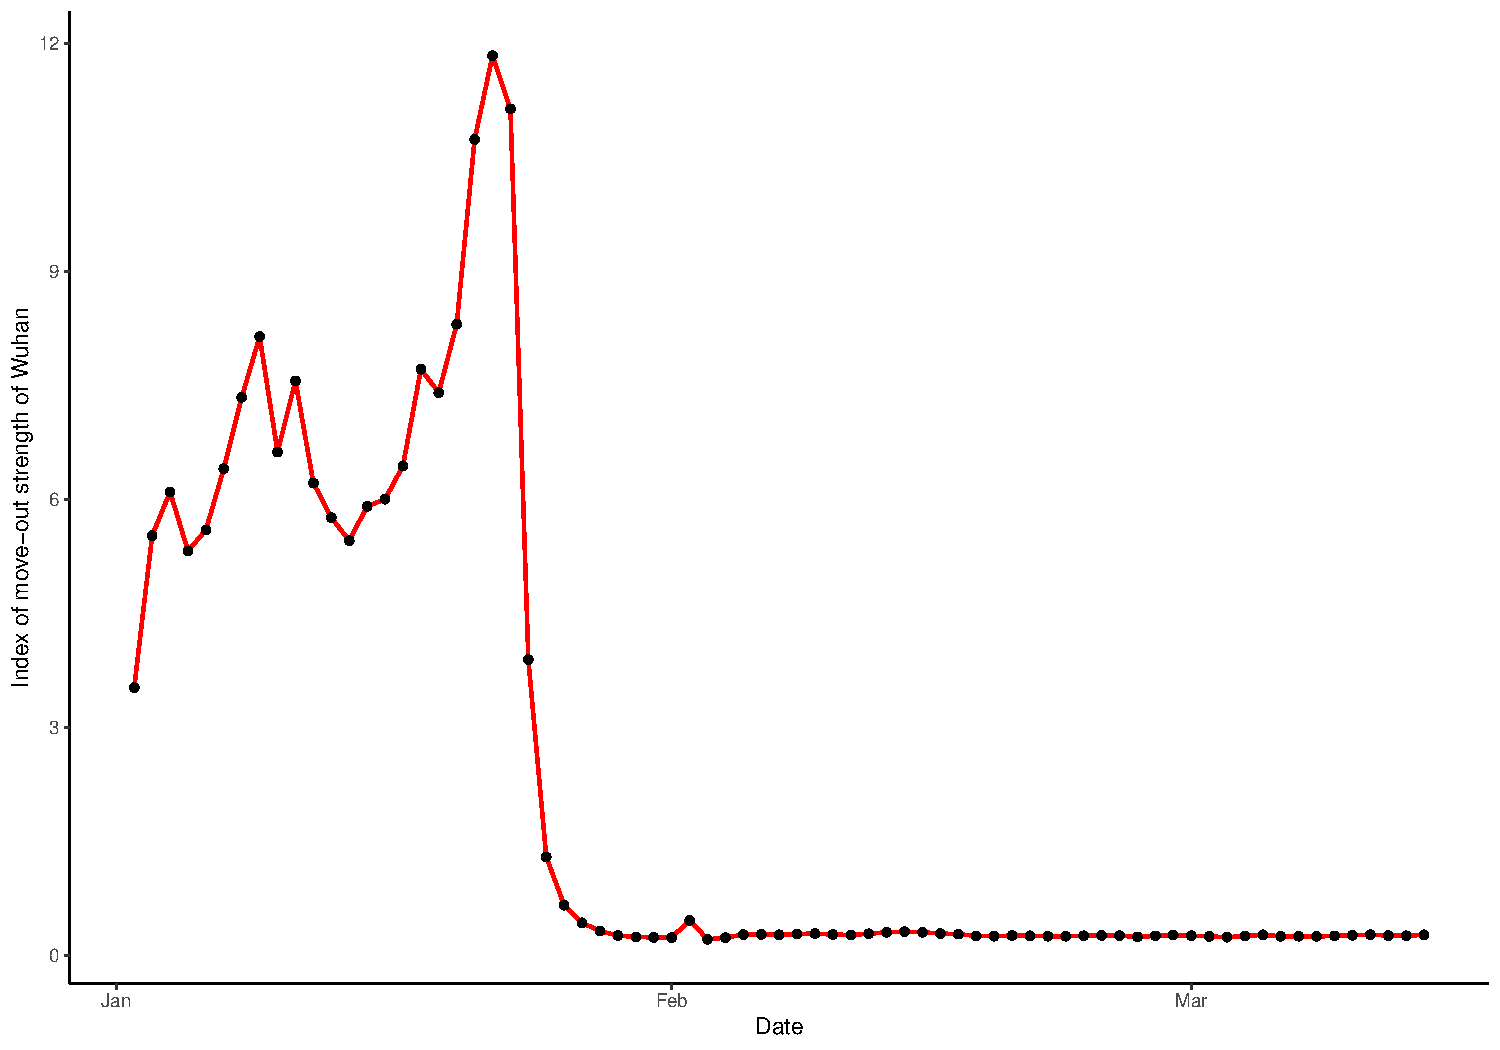
\includegraphics{slides_files/figure-beamer/fig1-1.pdf}
\caption{\label{fig:fig1}Move out trend from Wuhan}
\end{figure}

\end{frame}

\begin{frame}{Top move-out cities are all in Hubei province}
\protect\hypertarget{top-move-out-cities-are-all-in-hubei-province}{}

\begin{itemize}
\tightlist
\item
  Top move-out cities from Wuhan are all in Hubei province
\end{itemize}

\begin{figure}
\centering
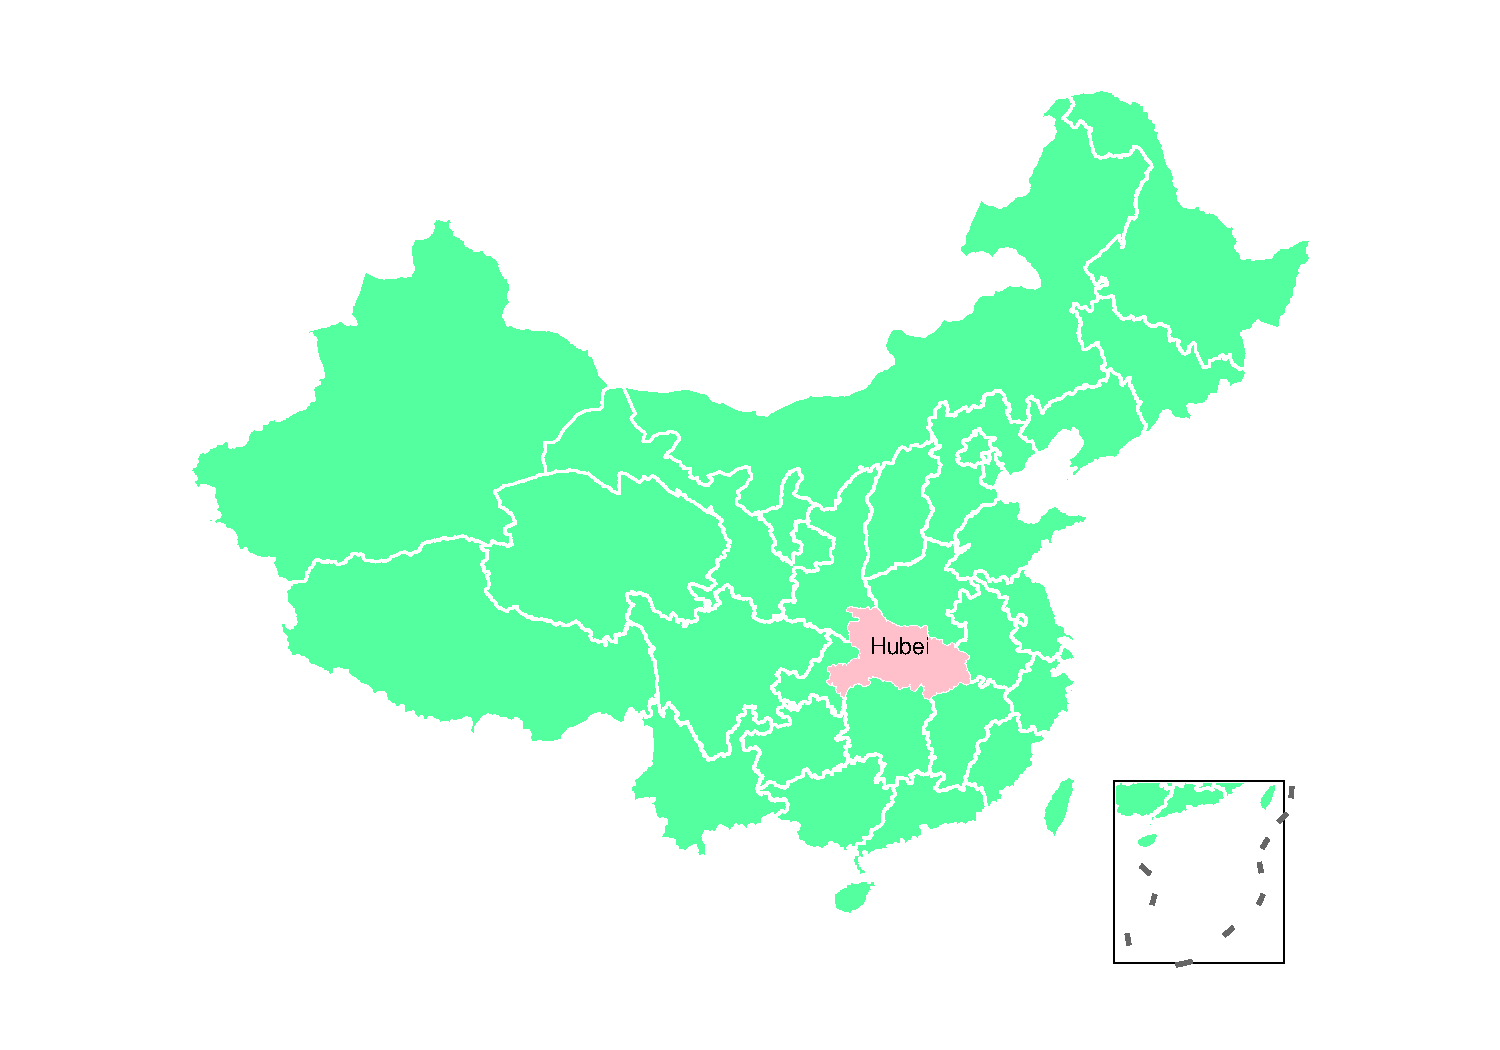
\includegraphics{slides_files/figure-beamer/fig2-1.pdf}
\caption{\label{fig:fig2}Hubei in China}
\end{figure}

\end{frame}

\begin{frame}{Hygienie of city and epidemic outbreak}
\protect\hypertarget{hygienie-of-city-and-epidemic-outbreak}{}

\begin{figure}
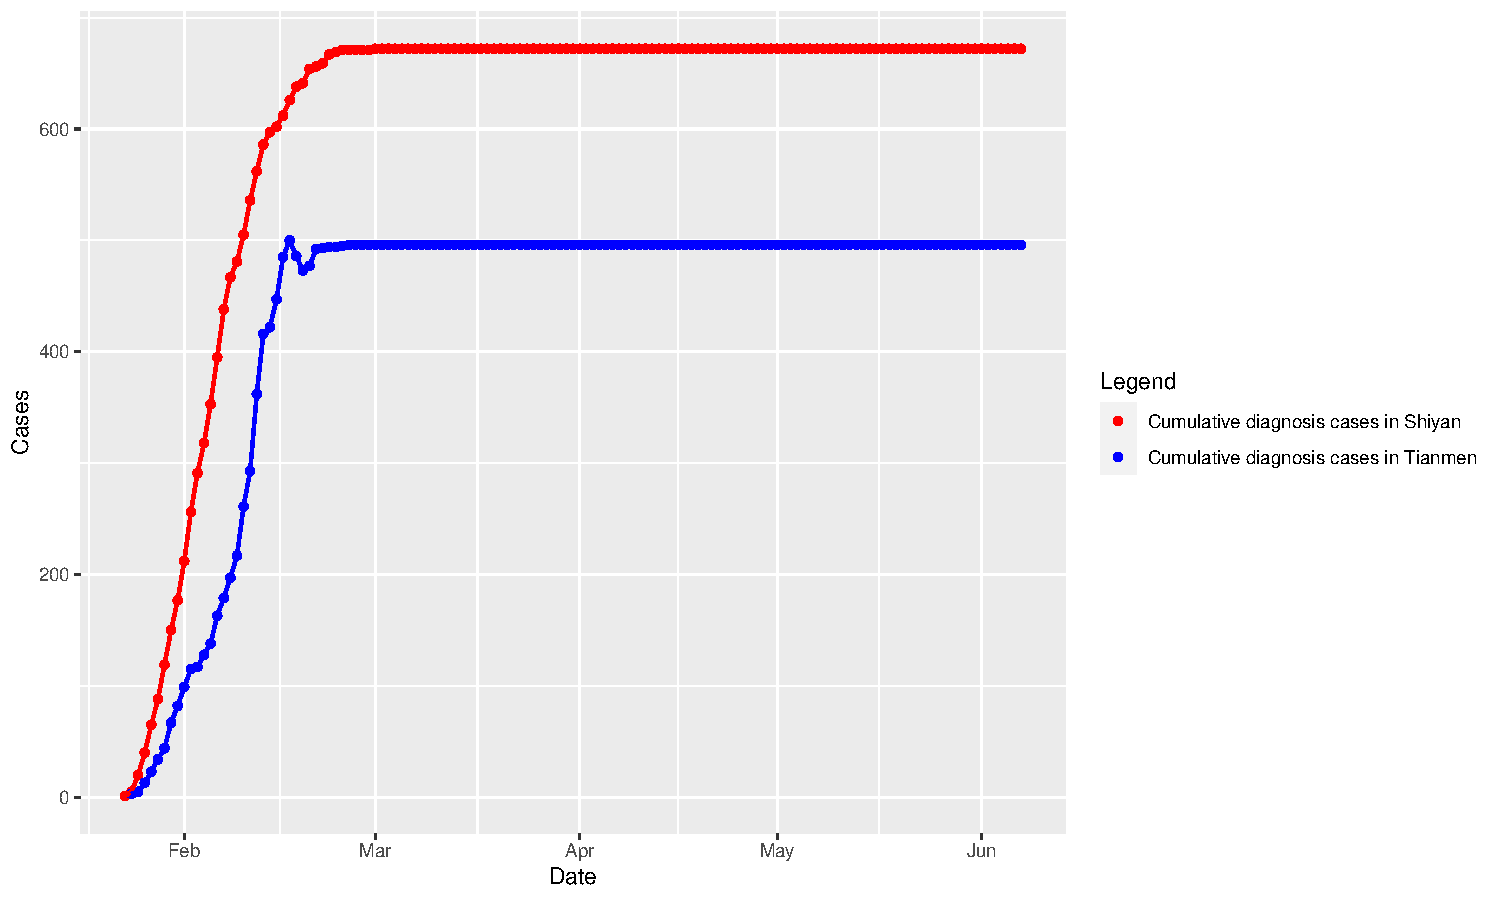
\includegraphics[width=1\linewidth]{slides_files/figure-beamer/fig3-1} \caption{A comparision of Tianmen and Shiyan}\label{fig:fig3}
\end{figure}

\end{frame}

\begin{frame}{All cities outside Wuhan}
\protect\hypertarget{all-cities-outside-wuhan}{}

\begin{figure}
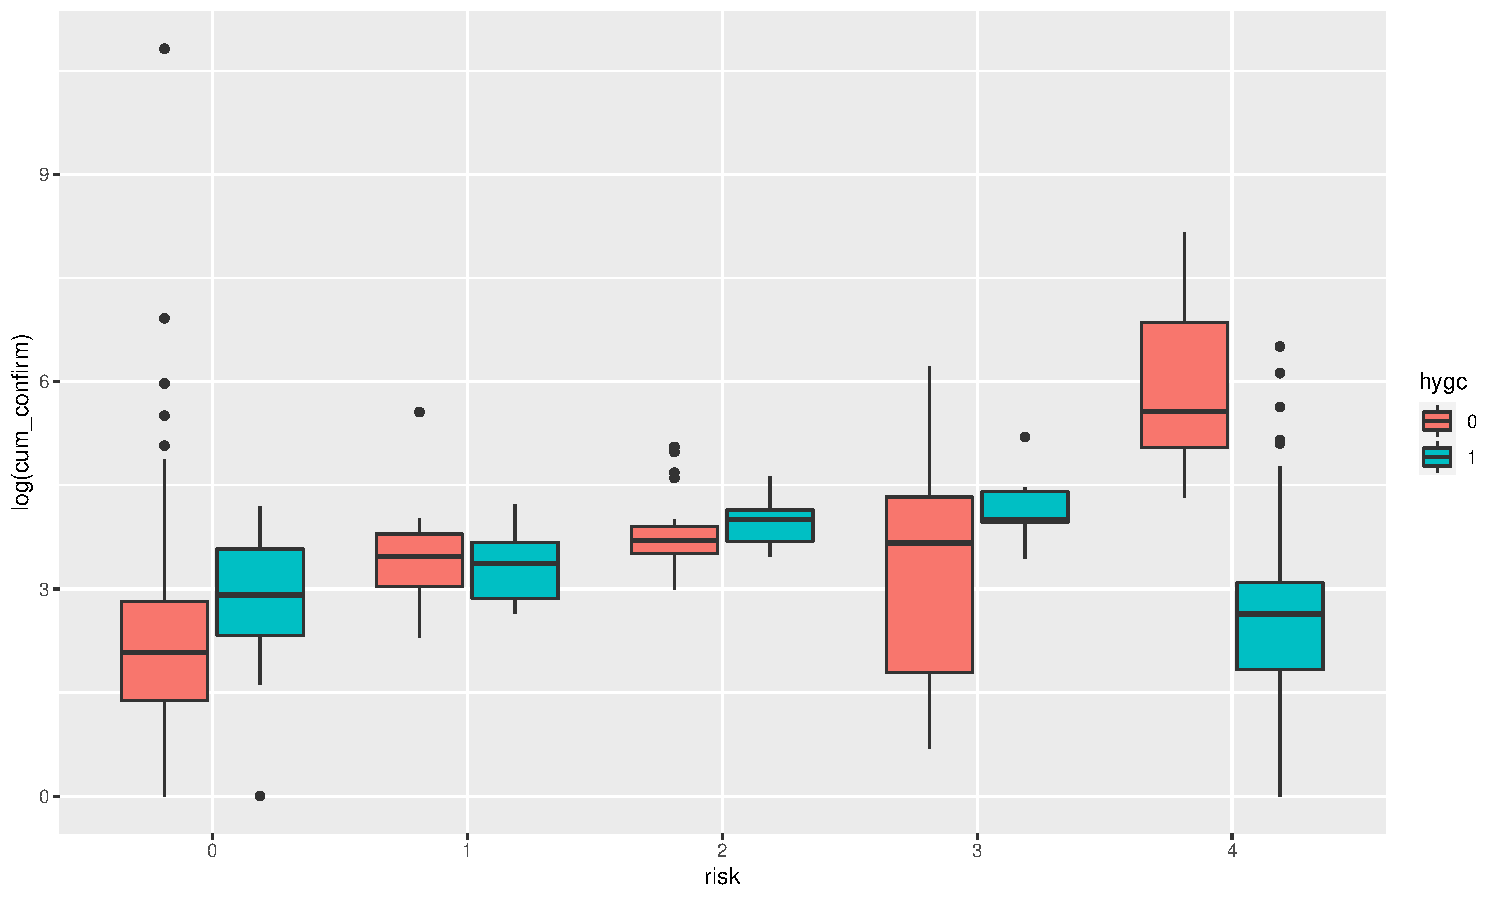
\includegraphics[width=1\linewidth]{slides_files/figure-beamer/fig4-1} \caption{A comparision of all cities outside Wuhan}\label{fig:fig4}
\end{figure}

\end{frame}

\begin{frame}{All cities outside Wuhan}
\protect\hypertarget{all-cities-outside-wuhan-1}{}

\begin{figure}
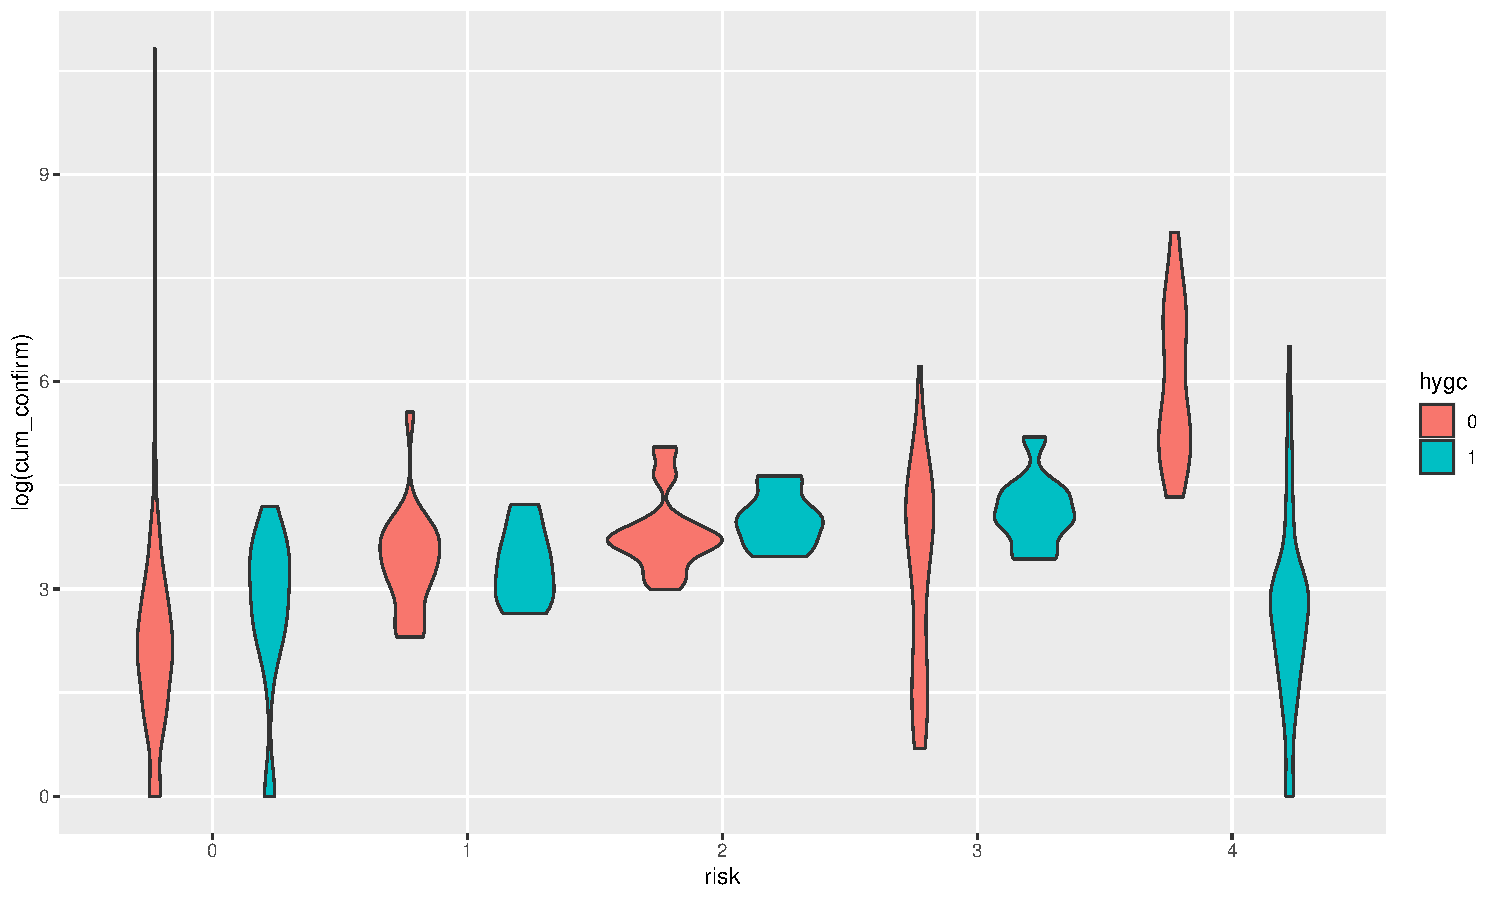
\includegraphics[width=1\linewidth]{slides_files/figure-beamer/fig5-1} \caption{A comparision of all cities outside Wuhan}\label{fig:fig5}
\end{figure}

\end{frame}

\hypertarget{summary}{%
\section{Summary}\label{summary}}

\begin{frame}{Conclusions}
\protect\hypertarget{conclusions}{}

\begin{itemize}
\item
  Lockdown of Wuhan City effectively cut-down the move-out from Wuhan City.
\item
  Top 10\% move-out cities from Jan 10,2020 to Jan 25,2020 are all in Hubei province
\item
  National hygienic city may not have a better control of the epidemic
\item
  However, the outliers with weak epidemic control, are more likely to be non- national hygienic city
\item
  Still ongoing\ldots{}
\end{itemize}

\end{frame}

\begin{frame}{Future work}
\protect\hypertarget{future-work}{}

\begin{itemize}
\tightlist
\item
  Multi-way ANOVA
\item
  Multiple linear regression
\item
  Mortality \& Inhospital time
\item
  Detailed hygiene condition
\end{itemize}

\end{frame}

\begin{frame}{Value and impact}
\protect\hypertarget{value-and-impact}{}

\textbf{Theorical implication}: how does hygiene impact the disease transmission, which will help to understand the transimission dynamics of the virus.

\textbf{Practical implication}: to evaluate the effectiveness of national hygienic cities, which will promote the city hygiene in China and beyond.

\end{frame}

\begin{frame}{Limitations}
\protect\hypertarget{limitations}{}

\begin{itemize}
\item
  The transmission may start from New Year travel in early January
\item
  The move-out data from Wuhan does not include transportation means
\item
  Real performance of local government varies in response to this emerging infectious disease
\end{itemize}

\end{frame}

\begin{frame}{Acknowledgement}
\protect\hypertarget{acknowledgement}{}

\begin{itemize}
\tightlist
\item
  Baidu Qianxi
\item
  ncovr and nCov2019 packages
\end{itemize}

\end{frame}

\begin{frame}{References}
\protect\hypertarget{references}{}

\begin{itemize}
\item
  Sievert, Carson. 2020. Interactive Web-Based Data Visualization with R, Plotly, and Shiny. Chapman; Hall/CRC. \url{https://plotly-r.com}.
\item
  Vanderkam, Dan, JJ Allaire, Jonathan Owen, Daniel Gromer, and Benoit Thieurmel. 2018. Dygraphs: Interface to 'Dygraphs' Interactive Time Series Charting Library. \url{https://CRAN.R-project.org/package=dygraphs}.
\item
  Wickham, Hadley. 2016. Ggplot2: Elegant Graphics for Data Analysis. Springer-Verlag New York. \url{https://ggplot2.tidyverse.org}.
\item
  Yu, Guangchuang. 2020. NCov2019: Stats of the '2019-nCov' Cases.
\item
  Zhao, Peng. 2019. Beginr: Functions for R Beginners. \url{https://CRAN.R-project.org/package=beginr}.
\item
  Zhao, Peng, Yi Zou, Lei Han, and Xinyuan Chu. 2020. Ncovr: Read and Process nCoV Data. \url{https://github.com/pzhaonet/ncovr}.
\end{itemize}

\end{frame}

\hypertarget{q-a}{%
\section{Q \& A}\label{q-a}}

\begin{frame}{I think you may ask?}
\protect\hypertarget{i-think-you-may-ask}{}

\textbf{Justification and Limitations}

Q1: How's the GDP's influence on the disease transmission?
A1: GDP may be related to move out data, and the move out data will be controlled adjusted in the data analysis.

Q2: Will the emerging public health response level in different city be an confounidng variable?
Q2: No, other than the lockdown of Wuhan city, the policy in China are relatively consistent. Each city announce their emergency public health response level according to national standard. \textbf{However, we don't know if the real performance varies in each city's local government, this will be an limitation}.

Q3: Will the rural infected cases and rural hygiene be included in the analysis
Q3: Yes, the assementent of national hygienic cities include the rural areas belong to this city. The rural infected cases also included in the total confirmed cases in a city.

\end{frame}

\begin{frame}{You may ask}
\protect\hypertarget{you-may-ask}{}

Q4: There is a time difference of the assement of national hygienic cities and epidemic outbreak, will it bias the results.
A4: Not likely, because the assement based the whole year performance in 2018 and published at March, 2019, which is the newest version. The epidemic outside mainly start transmission at Spring Festival travel in 2020. The hygiene of a city is the long-term efforts of local goverment and citizens, the change can be neglected to change within one year.

Q5: Will the transmission start from New Year travel in early January.
A5: \textbf{Maybe, this will be an limitation}

Q6: After the lockdown of Wuhan city, some people scape out Wuhan city secretly, will they be included in the move out data.
A6: It's difficult to know them, but we assume the number are not too much

\end{frame}

\end{document}
